\lab{Visualizing Complex-valued Functions}{Visualizing Complex-valued Functions}
\objective{Functions that map from the complex plane into the complex plane are difficult to fully visualize because the domain and range are both $2$-dimensional.
However, such functions can be visualized at the expense of partial information.
In this lab we present methods for analyzing complex-valued functions visually, including locating their zeros and poles in the complex plane.
We recommend completing the exercises in a Jupyter Notebook.}

\section*{Representations of Complex Numbers} % ===============================

A complex number $z = x+iy$ can be written in \emph{polar coordinates} as $z = re^{i\theta}$ where
\begin{itemize}
\item $r = |z| = \sqrt{x^2+y^2}$ is the \emph{magnitude} of $z$, and
\item $\theta = \arg(z) = \arctan(y/x)$ is the \emph{argument} of $z$, the angle in radians between $z$ and $0$.
\end{itemize}
Conversely, Euler's formula is the relation $re^{i\theta} = r\cos(\theta) + ir\sin(\theta)$.
Then setting $re^{i\theta}=x+iy$ and equating real and imaginary parts yields the equations $x=r\cos(\theta)$ and $y=r\sin(\theta)$.

\begin{figure}[H]
\begin{tikzpicture}[dot/.style={circle,fill=black,minimum size=3pt,
    inner sep=0pt,outer sep=-1pt}, >=stealth', thick, xscale=1.4]

\draw[-](-.5,0)--(3,0);
\draw[-](0,-.5)--(0,3);

\draw[-, dashed, gray, anchor=east](2.6,2.3)--(0,2.3);
\node[draw=none]()at(-.3,2.3){$iy$};
\draw[-, dashed, gray, anchor=north ](2.6,2.3)--(2.6,0);
\node[draw=none]()at(2.6,-.3){$x$};

\draw[gray](.75,0) arc (0:45:.7 and .7);

\draw[-](0,0)--(2.6,2.3);
\node[dot,draw](point)at(2.6,2.3){};
\node[draw=none]()at(2.8,2.5){$z$};
\node[draw=none]()at(.9,.35){$\theta$};

\draw [decorate,decoration={brace,amplitude=10pt},rotate=-45, gray] (0,0) --(.2,3.45);
\node[draw=none]()at(1.05,1.65){$r$};

\end{tikzpicture}
\caption{The complex number $z$ can be represented in Cartesian coordinates as $z = x+iy$ and in polar coordinates as $z = re^{i\theta}$, when $\theta$ is in radians.}
\label{fig:polar_coords}
\end{figure}

NumPy makes it easy to work with complex numbers and convert between coordinate systems.
The function \li{np.angle()} returns the argument $\theta$ of a complex number (between $-\pi$ and $\pi$) and \li{np.<<abs>>()} (or \li{np.absolute()}) returns the magnitude $r$.
These functions also operate element-wise on NumPy arrays.

\begin{lstlisting}
>>> import numpy as np

>>> z = 2 - 2*1j                    # 1j is the imaginary unit i = sqrt(-1).
>>> r, theta = np.<<abs>>(z), np.angle(z)
>>> print(r, theta)                 # The angle is between -pi and pi.
2.82842712475 -0.785398163397

# Check that z = r * e^(i*theta)
>>> np.isclose(z, r*np.exp(1j*theta))
<<True>>

# These function also work on entire arrays.
>>> np.<<abs>>(np.arange(5) + 2j*np.arange(5))
array([ 0.        ,  2.23606798,  4.47213595,  6.70820393,  8.94427191])
\end{lstlisting}

\section*{Complex Functions} % ================================================

A function $f: \mathbb{C} \rightarrow \mathbb{C}$ is called a \emph{complex-valued function}.
Visualizing $f$ is difficult because $\mathbb{C}$ has 2 real dimensions, so the graph of $f$ should be 4-dimensional.
However, since it is possible to visualize 3-dimensional objects, $f$ can be visualized by ignoring one dimension.
There are two main strategies for doing this: assign a color to each point $z\in\mathbb{C}$ corresponding to either the argument $\theta$ of $f(z)$, or to the magnitude $r$ of $f(z)$.
The graph that uses the argument is called a \emph{complex color wheel graph}.
Figure \ref{fig:complex-identity-angle-mag} displays the identity function $f(z) = z$ using these two methods.

\begin{figure}[H] % f(z) = z
\captionsetup[subfigure]{justification=centering}
\centering
\begin{subfigure}{.49\textwidth}
    \centering
    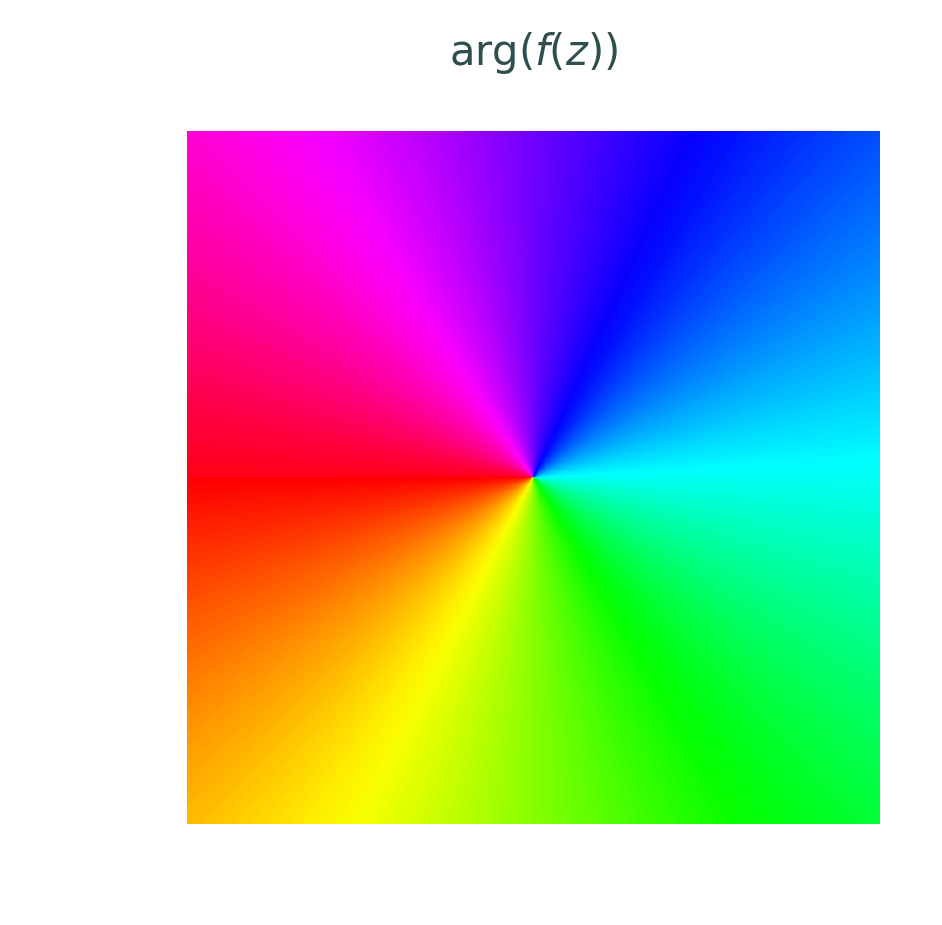
\includegraphics[width=\textwidth]{figures/identity_angle.png}
\end{subfigure}
%
\begin{subfigure}{.49\textwidth}
    \centering
    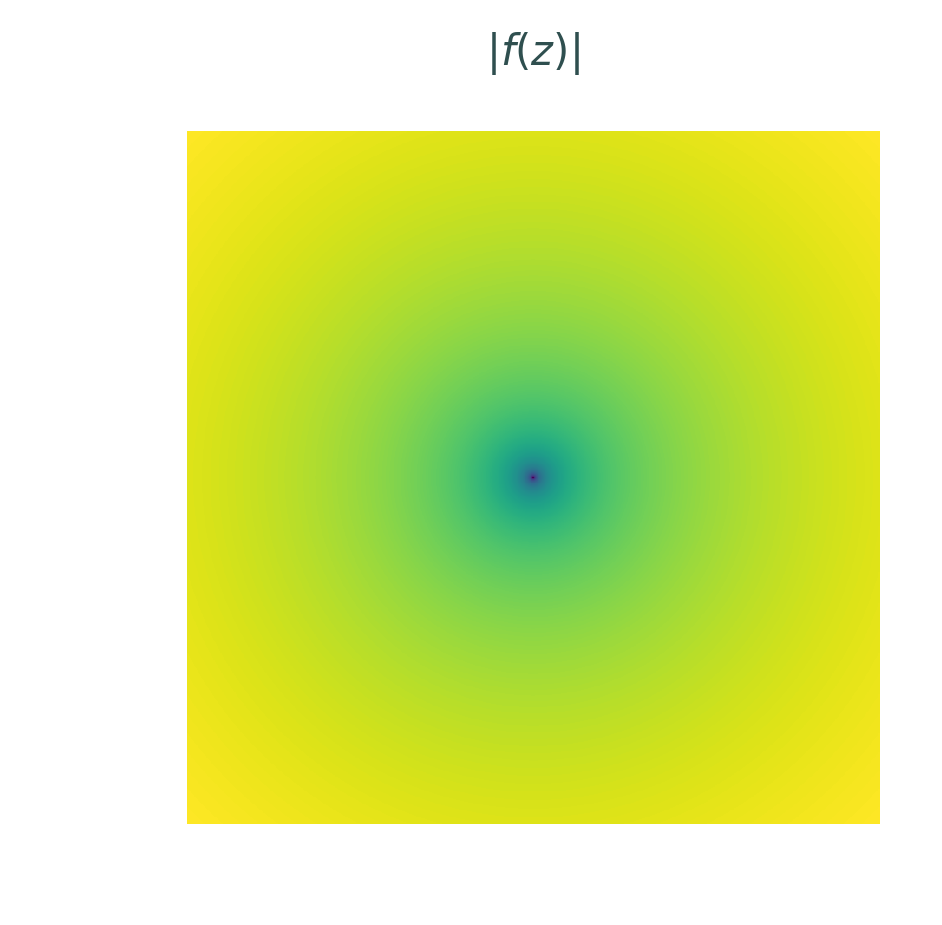
\includegraphics[width=\textwidth]{figures/identity_magnitude.png}
\end{subfigure}
\caption{The identity function $f: \mathbb{C} \rightarrow \mathbb{C}$ defined by $f(z)=z$. On the left, the color at each point $z$ represents the angle $\theta = \arg(f(z))$. As $\theta$ goes from $-\pi$ to $\pi$, the colors cycle smoothly counterclockwise from red to green to blue and back to red (this colormap is called \li{"hsv"}). On the right, the color represents the magnitude $r = |f(z)|$. The further a point is from the origin, the greater its magnitude (the colormap is the default, \li{"viridis"}).
}
\label{fig:complex-identity-angle-mag}
\end{figure}

The plots in Figure \ref{fig:complex-identity-angle-mag} use Cartesian coordinates in the domain and polar coordinates in the codomain.
The procedure for plotting in this way is fairly simple.
Begin by creating a grid of complex numbers: create the real and imaginary parts separately, then use \li{np.meshgrid()} to turn them into a single array of complex numbers.
Pass this array to the function $f$, compute the angle and argument of the resulting array, and plot them using \li{plt.pcolormesh()}.
The following code sets up the complex domain grid.

\begin{lstlisting}
>>> x = np.linspace(-1, 1, 400)     # Real domain.
>>> y = np.linspace(-1, 1, 400)     # Imaginary domain.
>>> X, Y = np.meshgrid(x, y)        # Make grid matrices.
>>> Z = X + 1j*Y                    # Combine the grids into a complex array.
\end{lstlisting}

Visualizing the argument and the magnitude separately provides different perspectives of the function $f$.
The angle plot is generally more useful for visualizing function behavior, though the magnitude plot often makes it easy to spot important points such as zeros and poles.
% Use both of these plots together to get as much information as possible about the function.

\begin{figure}[H] % f(z) = sqrt(z^2 - 1)
\captionsetup[subfigure]{justification=centering}
\centering
\begin{subfigure}{.49\textwidth}
    \centering
    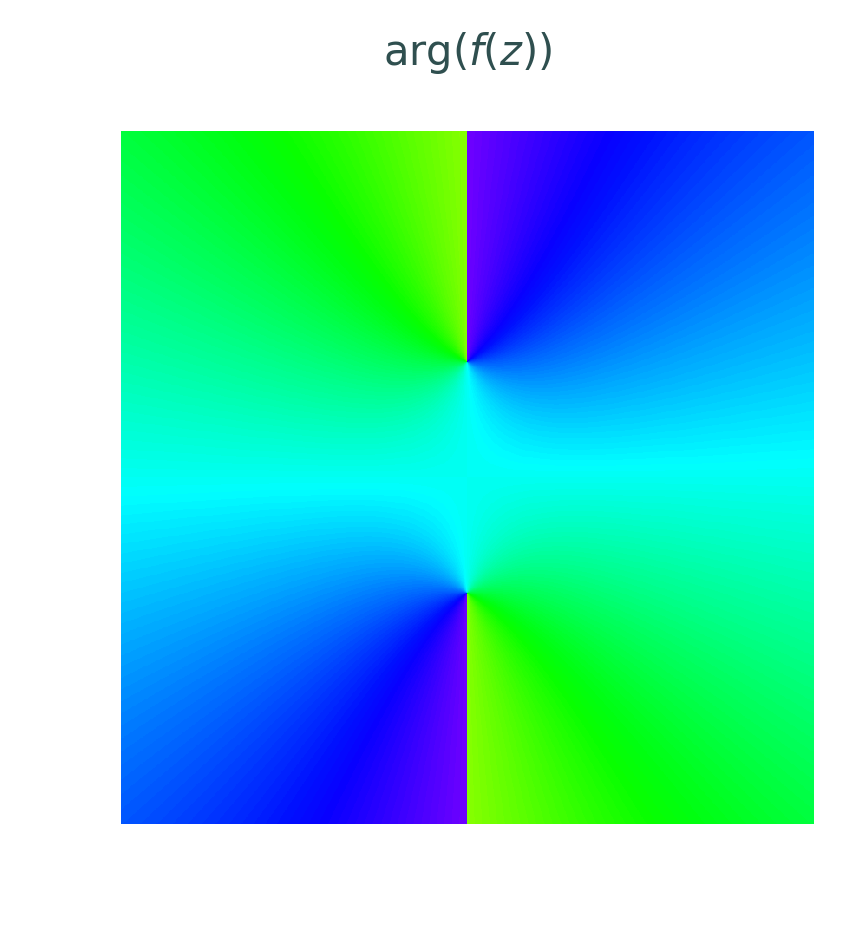
\includegraphics[width=\textwidth]{figures/discontinuity_angle.png}
\end{subfigure}
%
\begin{subfigure}{.49\textwidth}
    \centering
    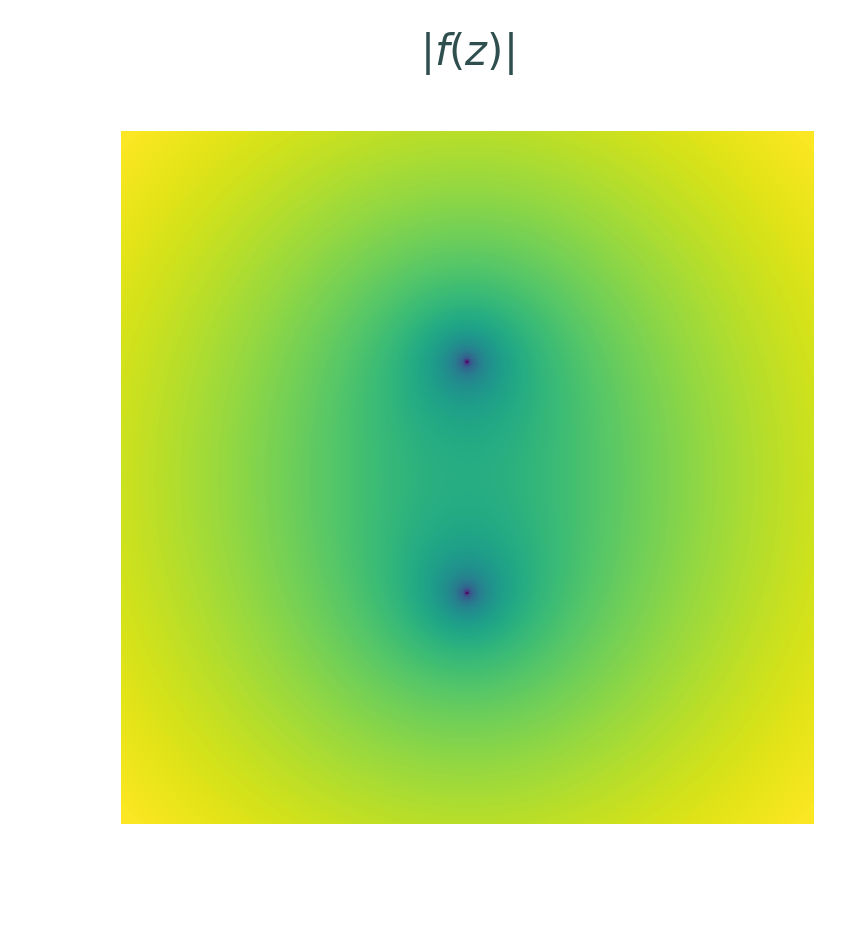
\includegraphics[width=\textwidth]{figures/discontinuity_magnitude.png}
\end{subfigure}
\caption{Plots of $f(z) = \sqrt{z^2+1}$ on $\{x+iy \mid x,y \in [-3,3]\}$.
Notice how a discontinuity is clearly visible in the angle plot on the left, but disappears from the magnitude plot on the right.}
\label{fig:complex-discontinuity}
\end{figure}

\begin{problem}
Write a function that accepts a function $f:\mathbb{C}\rightarrow\mathbb{C}$,  bounds $[r_{\text{min}},r_{\text{max}},i_{\text{min}},i_{\text{max}}]$ for the domain, an integer \li{res} that determines the resolution of the plot, and a string to set the figure title.
Plot $\arg(f(z))$ and $|f(z)|$ on an equally-spaced \li{res}$\times$\li{res} grid over the domain $\{x + iy \mid x \in [r_{\text{min}},r_{\text{max}}],\: y \in [i_{\text{min}},i_{\text{max}}]\}$ in separate subplots.
\begin{enumerate}
\item For $\arg(f(z))$, set the \li{plt.pcolormesh()} keyword arguments \li{vmin} and \li{vmax} to $-\pi$ and $\pi$, respectively.
This forces the color spectrum to work well with \li{np.angle()}.
Use the colormap \li{"hsv"}, which starts and ends red, so that the color is the same for $-\pi$ and $\pi$.

\item For $|f(z)|$, set \li{norm=matplotlib.colors.LogNorm()} in \li{plt.pcolormesh()} so that the color scale is logarithmic.
Use a sequential colormap like \li{"viridis"} or \li{"magma"}.

\item Set the aspect ratio to \li{"equal"} in each plot.
Give each subplot a title, and set the overall figure title with the given input string.
\end{enumerate}

Use your function to visualize $f(z) = z$ on $\{x+iy \mid x,y \in [-1,1]\}$ and $f(z) = \sqrt{z^2+1}$ on $\{x+iy \mid x,y \in [-3,3]\}$.
Compare the resulting plots to Figures \ref{fig:complex-identity-angle-mag} and \ref{fig:complex-discontinuity}, respectively.
\label{prob:complex-plotting-function}
\end{problem}

\section*{Interpreting Complex Plots} % =======================================

Plots of a complex function can be used to quickly identify important points in the function's domain.

\subsection*{Zeros} % ---------------------------------------------------------

A complex number $z_0$ is called a \emph{zero} of the complex-valued function $f$ if $f(z_0) = 0$.
% $z_0$ is also called a \emph{root} of the equation $f(z) = 0$.
The \emph{mutliplicity} or \emph{order} of $z_0$ is the largest integer $n$ such that $f$ can be written as $f(z) = (z - z_0)^n g(z)$ where $g(z_0) \ne 0$.
% In this case, $z_0$ is called a \emph{zero of order $n$} of $f$.
In other words, $f$ has a zero of order $n$ at $z_0$ if the Taylor series of $f$ centered at $z_0$ can be written as
\[
f(z) = \sum_{k=n}^{\infty} a_k(z-z_0)^k \qquad \text{with}\; a_n \neq 0.
\]

Angle and magnitude plots make it easy to locate a function's zeros and to determine their multiplicities.

\begin{problem} % Plot zeros.
Use your function from Problem \ref{prob:complex-plotting-function} to plot the following functions on the domain $\{x+iy \mid x,y \in [-1,1]\}$.
\begin{itemize}
\item $f(z) = z^n$ for $n=2,3,4$.
\item $f(z) = z^3 - iz^4 - 3z^6$.
Compare the resulting plots to Figure \ref{fig:complex-zeros}.
\end{itemize}
Write a sentence or two about how the zeros of a function appear in angle and magnitude plots.
How can you tell the multiplicity of the zero from the plot?
\label{prob:plot-complex-zeros}
\end{problem}

% In other words, $f(z) = a_n(z-z_0)^n + a_{n+1}(z-z_0)^{n+1} + \ldots$.
% This explains why we can estimate the order of a zero by counting the number of times the colors circle a point (see Figure \ref{fig:complex-zeros}).

Problem \ref{prob:plot-complex-zeros} shows that in an angle plot of $f(z) = z^n$, the colors cycle $n$ times counterclockwise around 0.
This is explained by looking at $z^n$ in polar coordinates.
\[
z^n = (re^{i \theta})^n = r^n e^{i(n\theta)}
\]
Multiplying $\theta$ by a number greater than $1$ compresses the graph along the ``$\theta$-axis'' by a factor of $n$.
In other words, the output angle repeats itself $n$ times in one cycle of $\theta$.
This is similar to taking a scalar-valued function $f:\mathbb{R}\rightarrow\mathbb{R}$ and replacing $f(x)$ with $f(nx)$.

Problem \ref{prob:plot-complex-zeros} also shows that the plot of $f(z) = z^3 - iz^4 - 3z^6$ looks very similar to the plot of $f(z) = z^3$ near the origin.
This is because when $z$ is close to the origin, $z^4$ and $z^6$ are much smaller in magnitude than $z^3$, and so the behavior of $z^3$ dominates the function.
In terms of the Taylor series centered at $z_0 = 0$, the quantity $|z-z_0|^{n+k}$ is much smaller than $|z-z_0|^n$ for $z$ close to $z_0$, and so the function behaves similar to $a_n(z-z_0)^n$.

\begin{figure}[H] % f(z) = z^3 - iz^4 - 3z^6
\captionsetup[subfigure]{justification=centering}
\centering
\begin{subfigure}{.49\textwidth}
    \centering
    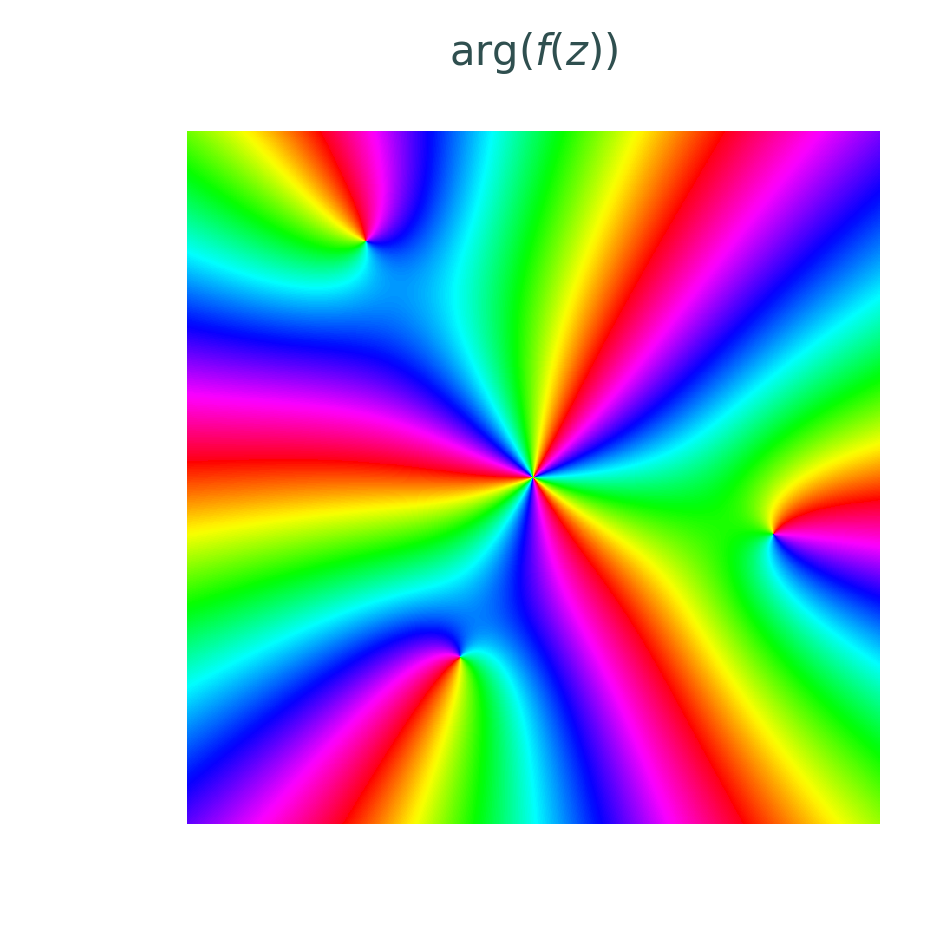
\includegraphics[width=\textwidth]{figures/zeros_angle.png}
\end{subfigure}
%
\begin{subfigure}{.49\textwidth}
    \centering
    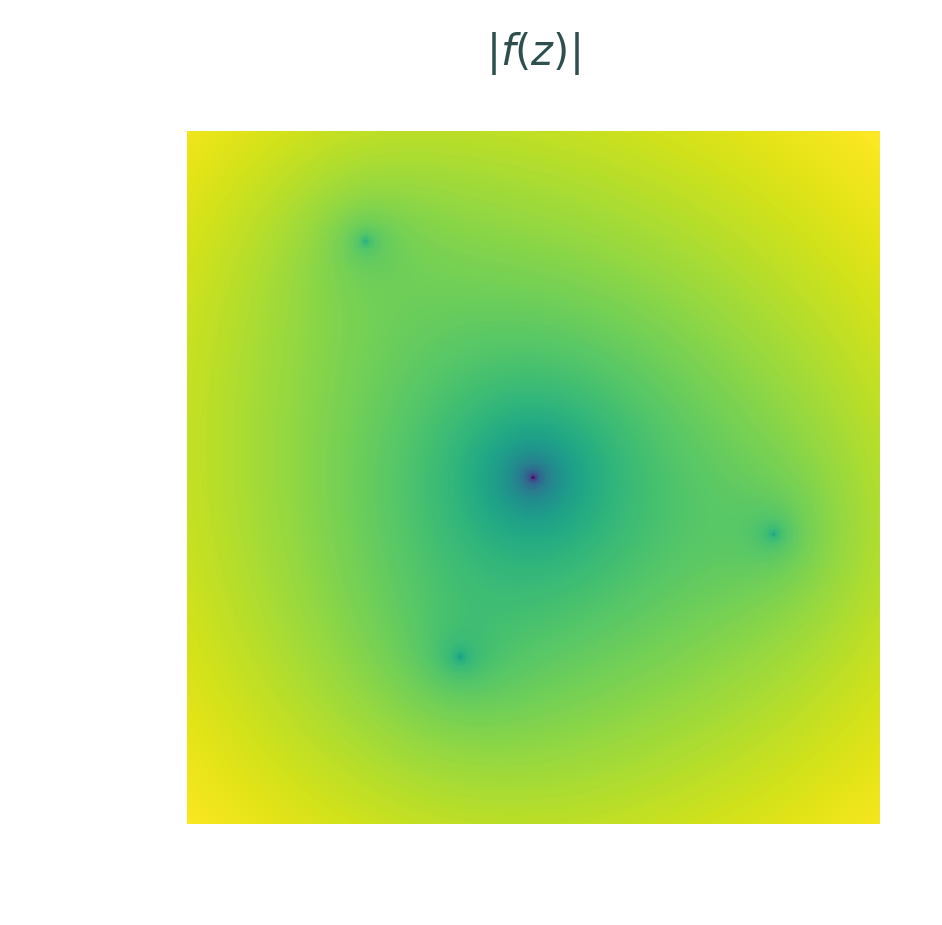
\includegraphics[width=\textwidth]{figures/zeros_magnitude.png}
\end{subfigure}
\caption{The angle plot of $f(z)=z^3 - iz^4 - 3z^6$ on $\{x+iy \mid x,y \in [-1,1]\}$. The angle plot shows that $f(z)$ has a zero of order $3$ at the origin and $3$ distinct zeros of order $1$ scattered around the origin.
The magnitude plot makes it easier to pinpoint the location of the zeros.}
% and shows that the basin around the origin is a little wider than the basins around the other zeros.}
\label{fig:complex-zeros}
\end{figure}

\subsection*{Poles} % ---------------------------------------------------------

A complex number $z_0$ is called a \emph{pole} of the complex-valued function $f$ if $f$ can be written as $f(z) = g(z) / (z - z_0)$ where $g(z_0) \ne 0$.
From this definition it is easy to see that $\lim_{z\rightarrow z_0}|f(z)| = \infty$, but knowing that $\lim_{z\rightarrow z_1}|f(z)| = \infty$ is not enough information to conclude that $z_1$ is a pole of $f$.

The \emph{order} of $z_0$ is the largest integer $n$ such that $f$ can be written as $f(z) = g(z) / (z - z_0)^n$ with $g(z_0) \ne 0$.
In other words, $f$ has a pole of order $n$ at $z_0$ if its Laurent series on a punctured neighborhood of $z_0$ can be written as
\[
f(z) = \sum_{k=-n}^\infty a_k(z-z_0)^k  \qquad \text{with} \; a_{-n} \neq 0.
\]

\begin{problem} % Plot poles.
Plot the following functions on domains that show all of its zeros and/or poles.
\begin{itemize}
\item $f(z) = z^{-n}$ for $n=1,2,3$.
\item $f(z) = z^2+iz^{-1}+z^{-3}$.
\end{itemize}
Write a sentence or two about how the poles of a function appear in angle and magnitude plots.
How can you tell the multiplicity of the poles from the plot?
\label{prob:plot-complex-poles}
\end{problem}

Problem \ref{prob:plot-complex-poles} shows that in angle plot of $z^{-1}$, the colors cycle $n$ times clockwise around $0$, as opposed to the counter-clockwise rotations seen around roots.
Again, this can be explained by looking at the polar representation.
\[
z^{-n} = (re^{i \theta})^{-n} = r^{-n} e^{i(-n\theta)}
\]
The minus sign on the $\theta$ reverses the direction of the colors, and the $n$ makes them cycle $n$ times.

From Problem \ref{prob:plot-complex-poles} it is also clear that $f(z) = z^2+iz^{-1}+z^{-3}$ behaves similarly to $z^{-3}$ for $z$ near the pole at $z_0 = 0$.
Since $|z-z_0|^{-n+k}$ is much smaller than $|z-z_0|^{-n}$ when $|z-z_0|$ is small, near $z_0$ the function behaves like $a_{-n}(z-z_0)^{-n}$.
This is why the order of a pole can be estimated by counting the number of times the colors circle a point in the clockwise direction.

\subsection*{Counting Zeros and Poles} % --------------------------------------

The \emph{Fundamental Theorem of Algebra} states that a polynomial $f$ with highest degree $n$ has exactly $n$ zeros, counting multiplicity.
For example, $f(z) = z^2 + 1$ has two zeros, and $f(z) = (z-i)^3$ has three zeros, all at $z_0 = i$ (that is, $z_0=i$ is a zero with multiplicity $3$).

The number of poles of function can also be apparent if it can be written as a quotient of polynomials.
For example, $f(z) = z / (z+i)(z-i)^2$ has one zeros and three poles, counting multiplicity.

\begin{problem}
Plot the following functions and count the number and order of their zeros and poles.
Adjust the bounds of each plot until you have found all zeros and poles.
\begin{itemize}
\item $f(z) = -4z^5 + 2z^4 - 2z^3 - 4z^2 + 4z - 4$
\item $f(z) = z^7 + 6z^6 - 131z^5 - 419z^4 + 4906z^3 - 131z^2 - 420z + 4900$
\item $f(z) = \frac{16z^4 + 32z^3 + 32z^2 + 16z + 4}{16z^4 - 16z^3 + 5z^2}$
\end{itemize}
\end{problem}

It is usually fairly easy to see how many zeros or poles a polynomial or quotient of polynomials has.
However, it can be much more difficult to know how many zeros or poles a different function may or may not have without visualizing it.

\begin{problem}
\label{prob:findpz}
Plot the following functions on the domain $\{x+iy\mid x,y\in[-8,8]\}$.
Explain carefully what each graph reveals about the function and why the function behaves that way.
\begin{itemize}
\item $f(z) = e^z$
\item $f(z) = \tan(z)$
\end{itemize}
(Hint: use the polar coordinate representation to mathematically examine the magnitude and angle of each function.)
\end{problem}

\subsection*{Essential Poles} % -----------------------------------------------

A complex-valued function $f$ has an \emph{essential pole} at $z_0$ if its Laurent series in a punctured neighborhood of $z_0$ requires infinitely many terms with negative exponents.
For example,
\[
e^{1/z} = \sum_{k=0}^{\infty}\frac{1}{n! z^n} = 1+\frac{1}{z}+\frac{1}{2}\frac{1}{z^2}+\frac{1}{6}\frac{1}{z^3}+\ldots.
\]
An essential pole can be thought of as a pole of order $\infty$.
Therefore, in an angle plot the colors cycle infinitely many times around an essential pole.

\begin{figure}[H] % f(z) = e^(1/z)
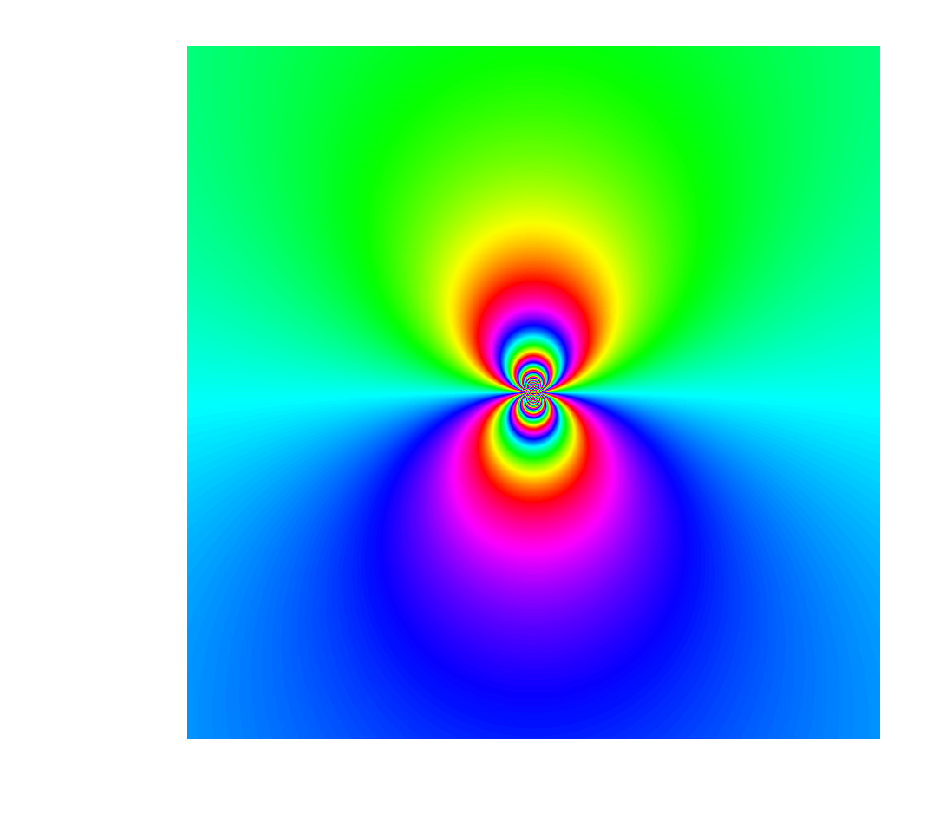
\includegraphics[width=.7\textwidth]{figures/poles_angle.png}
\caption{Angle plot of $f(z) = e^{1/z}$ on the domain $\{x+iy \mid x,y \in [-1,1]\}$.
The colors circle clockwise around the origin because it is a pole, not a zero.
Because the pole is essential, the colors repeat infinitely many times.}
\label{fig:complex-essential-pole}
\end{figure}

\begin{warn}
Often, color plots like the ones presented in this lab can be deceptive because of a bad choice of domain.
Be careful to validate your observations mathematically.
\end{warn}

\begin{problem}
For each of the following functions, plot the function on $\{x+iy\mid x,y\in[-1,1]\}$ and describe what this view of the plot seems to imply about the function.
Then plot the function on a domain that allows you to see the true nature of the roots and poles and describe how it is different from what the original plot implied.
\begin{itemize}
\item $f(z) = 100z^2 + z$
\item $f(z) = \sin\left(\frac{1}{100z}\right)$.
\end{itemize}
(Hint: zoom way in.)
\end{problem}


\begin{comment} % This part is confusing and not in the book.
\subsection*{Multi-Valued Functions} % ----------------------------------------

Every complex number has two complex square zeros, since if $w^2=z$, then also $(-w)^2=z$.
If $z$ is not zero, these zeros are distinct.

Over the nonnegative real numbers, it is possible to define a continuous square root function.
However, it is not possible to define a continuous square root function over any open set of the complex numbers that contains 0.
This is intuitive after graphing $\sqrt{z}$ on the complex plane.

\begin{problem}
Plot the following functions and explain why they look the way that they do.
\begin{itemize}
\item $f(z) = \sqrt{z}$.
Use \li{np.sqrt()} to take the square root.
\item $f(z) = -\sqrt{z}$.
\end{itemize}
\end{problem}

% Just as raising $z$ to a positive integer compresses the $\theta$-axis, making the color wheel repeat itself $n$ times around 0, raising $z$ to a fractional power \emph{stretches} the $\theta$-axis, so that only one $n^{th}$ of the color wheel appears around 0.
% The colors at the ends of this $n^{th}$-slice are not the same, but they appear next to each other in the plot of $z^{-n}$.
% This discontinuity will appear in every neighborhood of the origin.
%
% If your domain does not contain the origin, it is possible to define a continuous root function by picking one of the zeros.


\section*{Multi-Valued Functions} % -------------------------------------------

Another important topic in Complex Analysis is the study of multiple valued functions.
These functions arise as we consider the inverses of functions that are not strictly one to one on the complex plane.
A classic example is $\sqrt{x}$, which may take two values for every nonzero point of the complex plane.

In the Real numbers we worked with functions like this by simply restricting their output on a certain domain.
We can do a similar thing in the Complex plane.
Loosely speaking, such a restriction is called a branch.
Computationally we restrict the output to a single portion of the actual possible values of the multifunction.
Inverse functions that have multiple values like this are called \emph{multi-valued functions} or \emph{multifunctions}.
NumPy automatically restricts the output of multi-valued functions. So to get other cuts you have to modify the function to get the cut you want, like multiplying the output of the $\sqrt{x}$ by $-1$.
Figure \ref{fig:sqrt} shows the two cuts surfaces for $\sqrt{z}$ in the complex plane.

These are some very basic examples.
Another simple example is $\ln\left(z\right)$, which has a single value for the real part and infinitely many possible values for its imaginary part.
This is because for any complex $z\neq 0$, we have $e^z=e^{z+2n\pi}$ where $n$ is any integer.
\end{comment}

\begin{comment}
\begin{problem}
Write two functions, both accepting a natural number $n$.
Have one function plot the Riemann surface for the real part $f(z)=\sqrt[n]{z}$ and the other plot the imaginary part.

Hint: Convert $z$ in $f(z)=\sqrt[n]{z}$ to polar form as $z=re^{\theta + 2k\pi}$
If you then plug this into $\sqrt[n]{z}$ the function takes the form
\[f(z)=\sqrt[n]{r} e^{i \frac{\theta + 2 \pi k}{n}}\]
Notice that here $f(z)$ has distinct values for $k = 0, 1, \dots, n-1$ (a total of $n$ different values). Each value of $k$ corresponds to a different branch, which you can plot as $n$ separate surfaces.

If you use just one surface to plot each branch you will get erroneous vertical lines from jump discontinuities. Split each branch into two surfaces to get rid of these lines. You can investigate where the discontinuities occur by first plotting it as just one surface. The discontinuities happen at the same place for all $n$;
\end{problem}
\end{comment}


\begin{comment} % Integration. This has been orphaned.
\section*{Contour Integrals in the Complex Plane}

From multivariable calculus, you may recall that an integral may be taken along a path.
This is very similar to what can be done in the complex plane.
Consider the function $f(z)$ on the complex plane.
Let $z=x+iy$.
Let $u$ and $v$ be the real and imaginary parts of $f$ respectively.
We integrate $f$ along some contour $C$ in the complex plane, beginning at $z=a$ and ending at $z=b$.
This integral may be written
\[\int_c f(z)dz\]
Parameterizing $z$, we have
\[\int_a^b f\left( c\left(t\right)\right) c'\left(t\right) dt\]
Expanding into real and imaginary parts (where $c\left(t\right) = x\left(t\right) + i y\left(t\right)$), we have
\[\int_a^b \left(u \left(c \left(t\right)\right) x'\left(t\right)-v\left(c \left(t\right)\right) y'\left(t\right)\right) dt + i \int_a^b\left(v \left(c \left(t\right)\right)x'\left(t\right)+u\left(c \left(t\right)\right) y'\left(t\right)\right) dt\]
We have now written this complex integral as the sum of two real valued integrals in $\mathbb{R}$.
Note that this implies that $\int_C f(z) dz$ may depend on the contour we choose and not just on the endpoints $a$ and $b$.

\begin{problem}
Write a function which takes a complex function $f(z)$, a contour parameterization $c(t)$ of a contour $c$, and the integration bounds on $t$ and returns the integral of $f$ along the contour $c$.
Use the numerical integration function \li{sympy.mpmath.quad} and the numerical derivative function \li{sympy.mpmath.diff} included in mpmath (which is, in turn, included as a submodule of sympy).
These functions already work for complex numbers.
To do something similar with the integration routines in SciPy, we would have to separate the function into real and imaginary parts, as is shown above.

Using the function you just defined, integrate the following functions along the following contours
\begin{itemize}
\item $\bar{z}$ counterclockwise along the unit ball starting and ending at $1$
\item $\bar{z}$ along a straight line from $0$ to $1+i$
\item $\bar{z}$ along the real axis from $0$ to $1$, then along the line from $1$ to $1+i$
\item $\bar{z}$ along the unit ball centered at $i$ from $0$ to $1+i$
\item $e^z$ counterclockwise along the unit ball starting and ending at $1$
\item $e^z$ along a straight line from $0$ to $1+i$
\item $e^z$ along the real axis from $0$ to $1$, then along the line from $1$ to $1+i$
\item $e^z$ along the unit ball centered at $i$ from $0$ to $1+i$
\end{itemize}
\end{problem}

Notice that, for a holomorphic function on a simply connected domain, the integrals from one point to another are not path dependent for any contours that lie within the domain.
An immediate consequence of the theorem is that for a complex function $f$, holomorphic on a simply connected domain $D$, and a contour $C$ lying entirely within $D$ which begins and ends at some point $a\in D$,
\[\int_C f(z)dz=0\]

The quadrature algorithms used in many of the integration algorithms work along a straight line between the integration bounds in the complex plane, so for holomorphic functions we should be able to use the integration function we wrote earlier.
For example, integrating $e^z$ from $-1-i$ to $1+i$ can be done numerically like this:
\begin{lstlisting}
from sympy import mpmath as mp
mp.quad(lambda z: mp.exp(z), (complex(-1, -1), complex(1, 1)))
\end{lstlisting}

\section*{The Cauchy Integral Formula}

Another major theorem in complex analysis is called Cauchy's Integral Formula (not to be confused with Cauchy's Integral Theorem).
It states that for a domain $D$ in the complex plane, containing some contour $C$ and the interior of $C$, for any $z_0$ in the interior of $C$,
\[f(z_0)=\frac{1}{2\pi i} \int_C \frac{f(z)}{z-z_0} dz\]

With more work, this theorem can be used to show that any function $f$ holomorphic on some domain $D$ is also infinitely differentiable on that domain.
In fact, the $n$th derivative of $f$ is given by the formula
\[f^{(n)}(z_0) = \frac{n!}{2\pi i} \int_C \frac{f(z)}{(z-z_0)^{n+1}} dz\]
This result is also important because it allows us to relate the value of $f$ on the inside of a contour to the value of $f$ on the contour itself.
In other words, the values of $f$ inside the contour depend only on the values of $f$ along the contour itself.
A related theorem (the Morera theorem) states that if some function $f$ is continuous on a domain $D$ and for every contour beginning and ending at the same point, the formula $\int_C f(z) dz = 0$ holds, then $f$ is holomorphic on $D$.

\begin{problem}
Using Cauchy's Integral Formula, write a python function which returns a callable function which evaluates a complex function $f$ along the interior of a contour $C$.
It should accept a callable function for the parameterization of $C$, a callable function for the values of $f$ along $C$, and the bounds on the parameter used.
Assume in your function that $C$ begins and ends at the same point and that $f$ also begins and ends at the same value (so that $f$ is continuous along $C$)
Try it out on simple functions like $e^x$ with complex values and compare what you get with what calling the functions normally gives you.
\end{problem}

Notice that in Cauchy's Integral Formula, we are integrating along a contour that begins and ends at the same point.
The function is also holomorphic at every point except $z_0$. At $z_0$ the integrand is undefined and has a singularity.
This integral around a singularity has some useful properties.
We will discuss these properties later on.

\end{comment}


\begin{comment}
\section*{Appendix}
It is possible to visualize the argument and the modulus of the output of a complex function $f(z)$.
One way to do so is to assign the modulus to a \emph{lightness} of color.
For example, suppose we have a complex number with argument 0, so it will map to red in the color plots described above.
If its modulus is very small, then we can map it to a blackish red, and if its modulus is large, we can map it to a whitish red.
With this extra rule, our complex plots will still be very much the same, except that zeros will look like black dots and poles will look like white dots (see Figure \ref{fig:example} for an example).

The code below implements the map we just described.
Be warned that this implementation does not scale well.
For example, if you try to plot a complex function whose outputs are all very small in modulus, the entire plot will appear black.


\begin{lstlisting}
import numpy as np
import matplotlib.pyplot as plt
from colorsys import hls_to_rgb

def colorize(z):
    '''
    Map a complex number to a color (or hue) and lightness.

    INPUT:
    z - an array of complex numbers in rectangular coordinates

    OUTPUT:
    If z is an n x m array, return an n x m x 3 array whose third axis encodes
    (hue, lightness, saturation) tuples for each entry in z. This new array can
    be plotted by plt.imshow().
    '''

    zy=np.flipud(z)
    r = np.abs(zy)
    arg = np.angle(zy)

    # Define hue (h), lightness (l), and saturation (s)
    # Saturation is constant in our visualizations
    h = (arg + np.pi)  / (2 * np.pi) + 0.5
    l = 1.0 - 1.0/(1.0 + r**0.3)
    s = 0.8

    # Convert the HLS values to RGB values.
    # This operation returns a tuple of shape (3,n,m).
    c = np.vectorize(hls_to_rgb) (h,l,s)

    # Convert c to an array and change the shape to (n,m,3)
    c = np.array(c)
    c = c.swapaxes(0,2)
    c = c.swapaxes(0,1)
    return c
\end{lstlisting}

The following code uses the \li{colorize()} function to plot  $\frac{z^2 - 1}{z}$. The output is Figure \ref{fig:example}.

\begin{lstlisting}
>>> f = lambda z :  (z**2-1)/z
>>> x = np.linspace(-.5, 1.5, 401)
>>> y = np.linspace(-1, 1, 401)
>>> X,Y = np.meshgrid(x,y)
>>> Z=f(X+Y*1j)
>>> Zc=colorize(Z)
>>> plt.imshow(Zc, extent=(-.5, 1.5, -1, 1))
>>> plt.show()
\end{lstlisting}

\begin{figure}
\includegraphics[width=.7\textwidth]{figures/example.png}
\caption{Plot of the function $\frac{z^2 - 1}{z}$ created with \li{colorize()}.
Notice that the zero at 1 is a black dot and the pole at 0 is a white dot.}
\label{fig:example}
\end{figure}
\end{comment}
